\documentclass[12pt, a4paper, oneside]{ctexart}
\usepackage[margin=2cm]{geometry}%要先设置页边距,否则页眉页脚会偏
\usepackage{amsmath, amsthm, amssymb, bm, graphicx, hyperref, mathrsfs,float,xcolor,color}
\usepackage{listings}

% 用来设置附录中代码的样式

\lstset{
    basicstyle          =   \bf \ttfamily,          % 基本代码风格
    keywordstyle        =   \bfseries,   % 关键字风格
    keywordstyle        =   \color{blue},
    stringstyle         =   \color{magenta},
    commentstyle        =   \color{red}\ttfamily,
    language            =    [x86masm]Assembler,
    commentstyle        =   \rmfamily\itshape,  % 注释的风格,斜体
    escapeinside=``, % 英文分号中可写入中文
    stringstyle         =   \ttfamily,  % 字符串风格
    columns=fullflexible,%可以自动换行
    breaklines=true,%在单词边界处换行。
    numbers             =   left,   % 行号的位置在左边
    showspaces          =   false,  % 是否显示空格,显示了有点乱,所以不现实了
    numberstyle         =   \zihao{-5}\ttfamily,    % 行号的样式,小五号,tt等宽字体
    showstringspaces    =   false,
    captionpos          =   t,      % 这段代码的名字所呈现的位置,t指的是top上面
    frame               =   lrtb,   % 显示边框
}
\title{实验四 \qquad  时钟实验}
\author{学号:61822313 \qquad 姓名:钟锦程 \qquad 实验日期:\today}
\date{}
\begin{document}
\maketitle
\section{实验任务和实验结果}
\subsection{基础实验任务}
执行时钟程序时,屏幕上显示提示符':' ,由键盘输入当前时、分和秒值,即 XX:XX:XX↙,
随即显示时间,并不停地计时。当有键按下时,立即停止计时,返回 DOS。
\subsubsection{调试通过的源程序}
\begin{lstlisting}
DATA SEGMENT
    TIME DB 9 ;存放时间ASCII码的缓冲区
         DB ?
         DB 9 DUP(0)
    D2 DB 0DH,0AH,'$';0D是光标移到行首,0A是换行
    D3 DB 0AH,'$'
DATA ENDS
CODE SEGMENT
    ASSUME DS:DATA,CS:CODE 
START:
    MOV AX,DATA
    MOV DS,AX
    MOV AH,2;显示冒号
    MOV DL,':'
    INT 21H
    LEA DX,TIME;让用户输入时间XX:XX:XX
    MOV AH,0AH
    INT 21H
    MOV SI,OFFSET TIME ;ASCII TO BCD
    MOV AL,0
    MOV [SI+10],AL ;删掉缓冲区其余部分的内容
    MOV DX,OFFSET D3 ;将光标移到下一行,否则第一次输出会覆盖之前的内容
    MOV AH,9
    INT 21H
NEXT:
    MOV CH,[SI+2];HOUR(ASCII)TO BCD 存放在CH
    AND CH,0FH 
    MOV CL,4 
    SHL CH,CL 
    MOV BL,[SI+3]
    AND BL,0FH 
    ADD CH,BL 
    MOV DH,[SI+5];MINUTE(ASCII)TO BCD 存放在DH
    AND DH,0FH 
    SHL DH,CL 
    MOV BL,[SI+6]
    AND BL,0FH 
    ADD DH,BL 
    MOV DL,[SI+8];SECEND(ASCII)TO BCD 存放在DL
    AND DL,0FH 
    SHL DL,CL 
    MOV BL,[SI+9]
    AND BL,0FH 
    ADD DL,BL 
    CALL DELAY 
    MOV AL,DL ;秒值增1
    ADD AL,1
    DAA 
    MOV DL,AL
    CMP DL,60H;秒值与60比较,如果不等于则直接显示
    JNZ SHOW 
    MOV DL,00H ;秒置零
    MOV AL,DH 
    ADD AL,1 ;分钟+1
    DAA 
    MOV DH,AL 
    CMP DH,60H;分钟值与60比较,如果不等于则直接显示
    JNZ SHOW 
    MOV DH,00H;分钟置零
    MOV AL,CH;小时+1
    ADD AL,1
    DAA 
    MOV CH,AL 
    CMP CH,24H ;小时值与24比较,如果不等于则直接显示
    JNZ SHOW 
    MOV CH,00H;若小时值等于24,则置零后再转显示
    JMP SHOW
SHOW:
    MOV CL,4
    MOV AX,0000H;小时从BCD转换为ASCII并存到缓冲区
    MOV AL,CH 
    SHL AX,CL 
    SHR AL,CL 
    OR AX,3030H
    XCHG AH,AL
    MOV [SI+2],AX 
    MOV AX,0000H;分钟从BCD转换为ASCII并存到缓冲区
    MOV AL,DH 
    SHL AX,CL 
    SHR AL,CL 
    OR AX,3030H
    XCHG AH,AL
    MOV [SI+5],AX 
    MOV AX,0000H;秒从BCD转换为ASCII并存到缓冲区
    MOV AL,DL 
    SHL AX,CL 
    SHR AL,CL 
    OR AX,3030H
    XCHG AH,AL
    MOV [SI+8],AX 
    MOV DX,OFFSET TIME;输出到屏幕
    ADD DX,2;指向小时值开头的地址
    MOV AH,9
    INT 21H
    MOV AH,06;检查是否有键按下
    MOV DL,0FFH 
    INT 21H
    JNZ EXIT
    JMP NEXT
EXIT:
    MOV AH,4CH ;若有键按下,结束程序
    INT 21H

DELAY PROC
    PUSH CX;保护可能改变的寄存器
    PUSH DX
    PUSH AX
    MOV AH,2CH;读取系统时间,DH得到秒值
    INT 21H
    MOV AL,DH 
    ADD AL,1;手动+1,使AL表示下一秒
READTIME:
    MOV AH,2CH;读取时间DH得到秒
    INT 21H
    CMP DH,AL
    JNZ READTIME;若不等于下一秒,则再读取时间;若相等,则结束延时
    POP AX
    POP DX
    POP CX
    RET
    DELAY ENDP
CODE ENDS
    END START 
\end{lstlisting}
\subsubsection{实验结果}
如图\ref{实验1结果截图1}是刚打开程序时的显示,屏幕打印了一个冒号,并等待键盘输入。图\ref{实验1结果截图2}是输入时间23:59:55后的显示。截图第一排是输入的起始时间,自输入后,每隔一秒时间值加一秒并显示一次。在程序正常运行期间随机按下一个键,程序终止。截图最后一排显示程序已经停止,询问是否要留在DOSBox中。
\begin{figure}[H]
    \centering
    \begin{minipage}{0.45\textwidth}
    \centering
    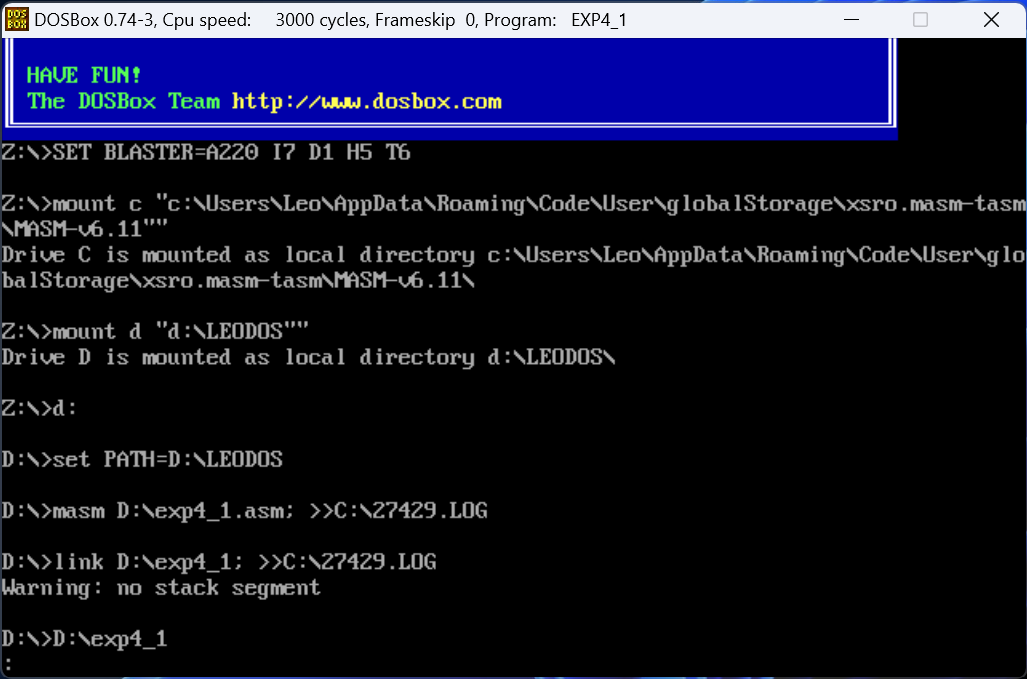
\includegraphics[scale=0.48]{pic/exp4-1-colon.png}
    \caption{基础实验任务结果截图1}
    \label{实验1结果截图1}
    \end{minipage}
    \hspace{0.05\textwidth}
    \begin{minipage}{0.45\textwidth}
    \centering
    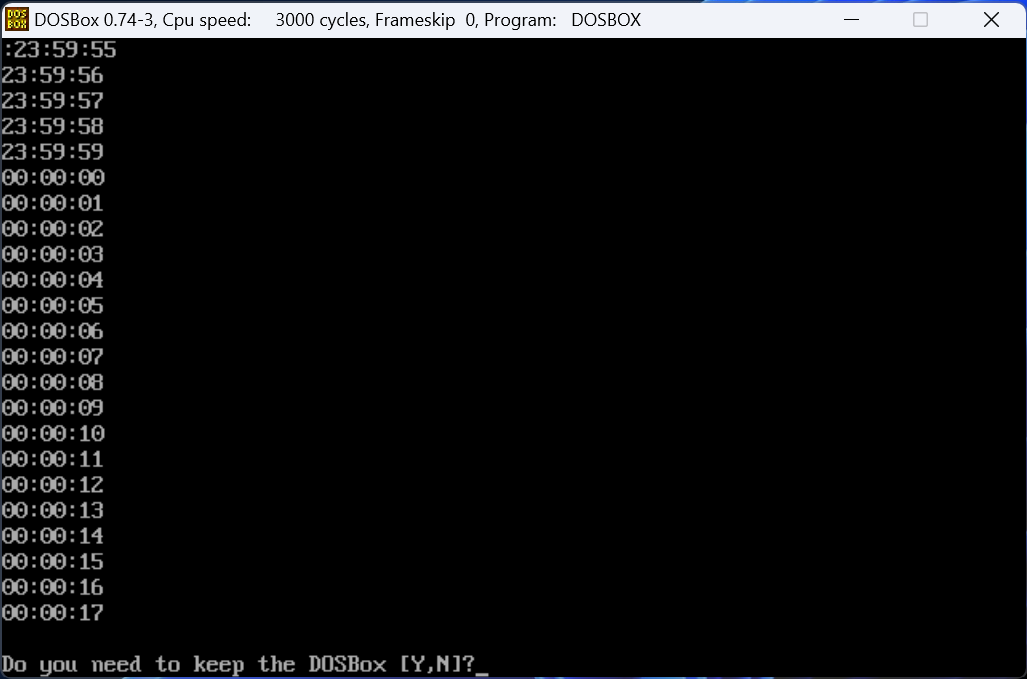
\includegraphics[scale=0.48]{pic/exp4-1-presskey.png}
    \caption{基础实验任务结果截图2}
    \label{实验1结果截图2}
    \end{minipage}
\end{figure}
\subsection{附加实验任务}
\begin{enumerate}
    \item 在同一行的相同位置显示更新的计时时间,不换行。
    \item 输入时间初值时,能够检查是否存在错误、提示错误信息,并可重新输入时间初值。
    错误类型及提示信息分为两种:
    1.输入的时间初值是错误的字符,即不是数字或冒号;
    2.输入的时间值是错误的,即“时”大于等于 24,“分”和“秒”大于等于 60。
    \item 延时一秒采用 DOS 系统功能调用实现
\end{enumerate}
\subsubsection{调试通过的源程序}
\begin{lstlisting}
DATA SEGMENT
    TIME DB 9 
         DB ?
         DB 9 DUP(0)
    D2 DB 0DH,'$';0D是光标移到行首,0A是换行
    D3 DB 0AH,'$'
    ERRINFO1 DB 0AH,'WRONG INFO 1:INPUT NOT NUMBER OR COLON',0DH,0AH,'$'
    ERRINFO2 DB 0AH,'WRONG INFO 2:INPUT TIME UNREASONABLE',0DH,0AH,'$'
    RETYPEINFO DB 'INPUT AGAIN:',0DH,0AH,'$'
DATA ENDS
CODE SEGMENT
    ASSUME DS:DATA,CS:CODE 
START:
    MOV AX,DATA
    MOV DS,AX
    MOV AH,2;显示冒号
    MOV DL,':'
    INT 21H
    MOV DX,OFFSET D3 
    MOV AH,9
    INT 21H    
    LEA DX,TIME;让用户输入时间XX:XX:XX
    MOV AH,0AH
    INT 21H
    MOV SI,OFFSET TIME 
    MOV AL,0
    MOV [SI+10],AL 
    CALL CHECK ;调用检查子程序。检查输入是否错误,提示错误信息,若错误,重新输入时间初值
NEXT:
    CALL ATOB;调用ASCII到BCD码的转换子程序
    CALL DELAY ;调用延时程序
    MOV AL,DL ;秒值增1
    ADD AL,1
    DAA 
    MOV DL,AL
    CMP DL,60H
    JNZ SHOW 
    MOV DL,00H ;秒置零
    MOV AL,DH 
    ADD AL,1 ;分钟+1
    DAA 
    MOV DH,AL 
    CMP DH,60H
    JNZ SHOW 
    MOV DH,00H;分钟置零
    MOV AL,CH;小时+1
    ADD AL,1
    DAA 
    MOV CH,AL 
    CMP CH,24H 
    JNZ SHOW 
    MOV CH,00H
    JMP SHOW
SHOW:
    MOV CL,4
    MOV AX,0000H;小时从BCD转换为ASCII并存到缓冲区
    MOV AL,CH 
    SHL AX,CL 
    SHR AL,CL 
    OR AX,3030H
    XCHG AH,AL
    MOV [SI+2],AX 
    MOV AX,0000H;分钟从BCD转换为ASCII并存到缓冲区
    MOV AL,DH 
    SHL AX,CL 
    SHR AL,CL 
    OR AX,3030H
    XCHG AH,AL
    MOV [SI+5],AX 
    MOV AX,0000H;秒从BCD转换为ASCII并存到缓冲区
    MOV AL,DL 
    SHL AX,CL 
    SHR AL,CL 
    OR AX,3030H
    XCHG AH,AL
    MOV [SI+8],AX 
    MOV DX,OFFSET TIME;输出到屏幕
    ADD DX,2
    MOV AH,9
    INT 21H
    MOV AH,06;检查是否有键按下
    MOV DL,0FFH 
    INT 21H
    JNZ EXIT
    JMP NEXT
EXIT:
    MOV AH,4CH ;若有键按下,结束程序
    INT 21H

ATOB PROC 
    MOV CH,[SI+2];HOUR(ASCII)TO BCD 存放在CH
    AND CH,0FH 
    MOV CL,4 
    SHL CH,CL 
    MOV BL,[SI+3]
    AND BL,0FH 
    ADD CH,BL 
    MOV DH,[SI+5];MINUTE(ASCII)TO BCD 存放在DH
    AND DH,0FH 
    SHL DH,CL 
    MOV BL,[SI+6]
    AND BL,0FH 
    ADD DH,BL 
    MOV DL,[SI+8];SECEND(ASCII)TO BCD 存放在DL
    AND DL,0FH 
    SHL DL,CL 
    MOV BL,[SI+9]
    AND BL,0FH 
    ADD DL,BL 
    RET ;不加RET会继续执行下面的DELAY,最终导致每次延时多一秒!
    ATOB ENDP
DELAY PROC;延时子程序
    PUSH CX
    PUSH DX
    PUSH AX
    MOV AH,2CH;读取时间DH得到秒
    INT 21H
    MOV AL,DH 
    ADD AL,1;AL表示下一秒
READTIME:
    MOV AH,2CH;读取时间DH得到秒
    INT 21H
    CMP DH,AL
    JNZ READTIME;若不等于下一秒,则再读取时间;若相等,则结束延时
    POP AX
    POP DX
    POP CX
    RET
    DELAY ENDP
CHECK PROC ;检查输入的子程序
    ;错误信息1:输入的时间不是数字或冒号
    ;错误信息2:输入的时间不符合实际
    ;此时SI已经指向TIME首址

    ;第一步:用ASCII码检查是不是数字或冒号
    PUSH CX;保护可能改变的寄存器
    PUSH AX
    PUSH DX
    PUSH BX
    MOV CX,8;置循环次数
    MOV BX,SI;把缓冲区首址复制给BX
    ADD BX,1
AGIN:
    MOV AX,SI
    ADD AX,4;AX用来指示冒号的位置
    INC BX;第一次循环开始时,BX(=SI+2)指到第一个字符,BX始终指向想要比较的字符
    CMP BX,AX;SI+4和SI+7指到冒号
    JZ CHECKCOLON;若指针指到冒号,则跳转冒号检查子程序
    ADD AX,3;指向下一个冒号
    CMP BX,AX
    JZ CHECKCOLON ;若指针指到冒号,则跳转冒号检查子程序
    JMP CHECKNUM ;两次都没有判定为指到冒号,说明是数字,跳转数字检查子程序
CHECKCOLON:;冒号检查
    CMP BYTE PTR [BX],':'
    JNZ WRONG1
    LOOP AGIN
CHECKNUM:;数字检查
    ;AX不能用来存放偏移地址!!!
    CMP BYTE PTR [BX],30H 
    JB WRONG1 
    CMP BYTE PTR [BX],39H
    JA WRONG1 
    LOOP AGIN 
    ;第二步:检查输入时间是否合理
    CALL ATOB ;调用ASCII到BCD的转换子程序。时分秒信息已经转换为BCD放到CH,DH,DL
    CMP CH,23H ;若小时数大于23,说明不合理,输出错误信息2
    JA WRONG2 
    CMP DH,59H;若分钟数大于59,说明不合理,输出错误信息2
    JA WRONG2 
    CMP DL,59H;若秒数大于59,说明不合理,输出错误信息2
    JA WRONG2 
    JMP OVER ;若不加这一句,无论如何都会执行WRONG1!!!
WRONG1:;输出错误信息1:输入的时间不是数字或冒号
    MOV DX,OFFSET ERRINFO1
    MOV AH,9
    INT 21H
    JMP RETYPE 
WRONG2:;输出错误信息2:输入的时间不符合实际
    MOV DX,OFFSET ERRINFO2
    MOV AH,9
    INT 21H
    JMP RETYPE
RETYPE:;提示重新输入并接收新的输入
    MOV DX,OFFSET RETYPEINFO
    MOV AH,9
    INT 21H
    LEA DX,TIME;让用户输入时间XX:XX:XX
    MOV AH,0AH
    INT 21H
    CALL CHECK
OVER:
    POP BX ;恢复现场
    POP DX
    POP AX
    POP CX 
    RET 
    CHECK ENDP
CODE ENDS
    END START 
\end{lstlisting}
\subsubsection{实验结果}
图\ref{附加实验任务结果截图1}是两种错误输入的结果。第一种错误输入:输入的不是数字或冒号。图中第一次在本应该输入数字的地方输入了字母a,程序显示了第一类错误信息并提示重新输入;第二次在本应该输入冒号的地方输入了分号,程序也显示了第一类错误信息并提示重新输入。第三次输入了一个不合理的时间值,即小时数大于23,程序输出了第二类错误信息并提示重新输入。图\ref{附加实验任务结果截图2}是正确规范的输入。输入后,每隔一秒在原位置更新时间值(没有换行),图\ref{附加实验任务结果截图3}显示了更新过程中的一个瞬间,表明时钟可以正常运行。最后,图\ref{附加实验任务结果截图4}显示:在程序运行过程中,在键盘上随便按一个键,可以让程序终止。
\begin{figure}[H]
    \centering
    \begin{minipage}{0.45\textwidth}
    \centering
    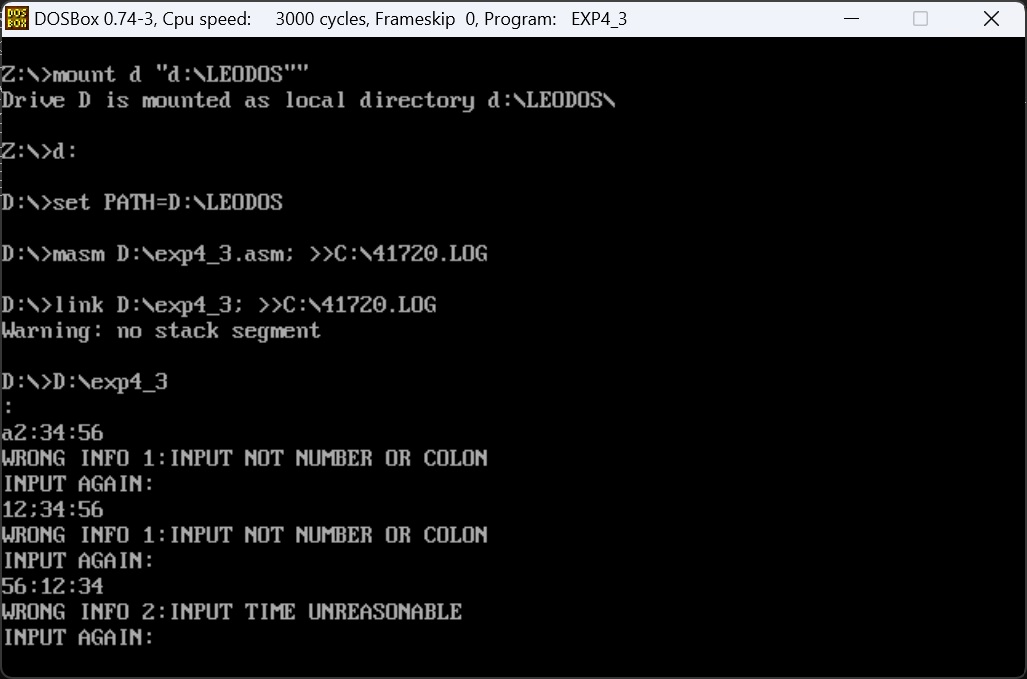
\includegraphics[scale=0.48]{pic/exp4-2-wronginfo.png}
    \caption{附加实验任务结果截图1}
    \label{附加实验任务结果截图1}
    \end{minipage}
    \hspace{0.05\textwidth}
    \begin{minipage}{0.45\textwidth}
    \centering
    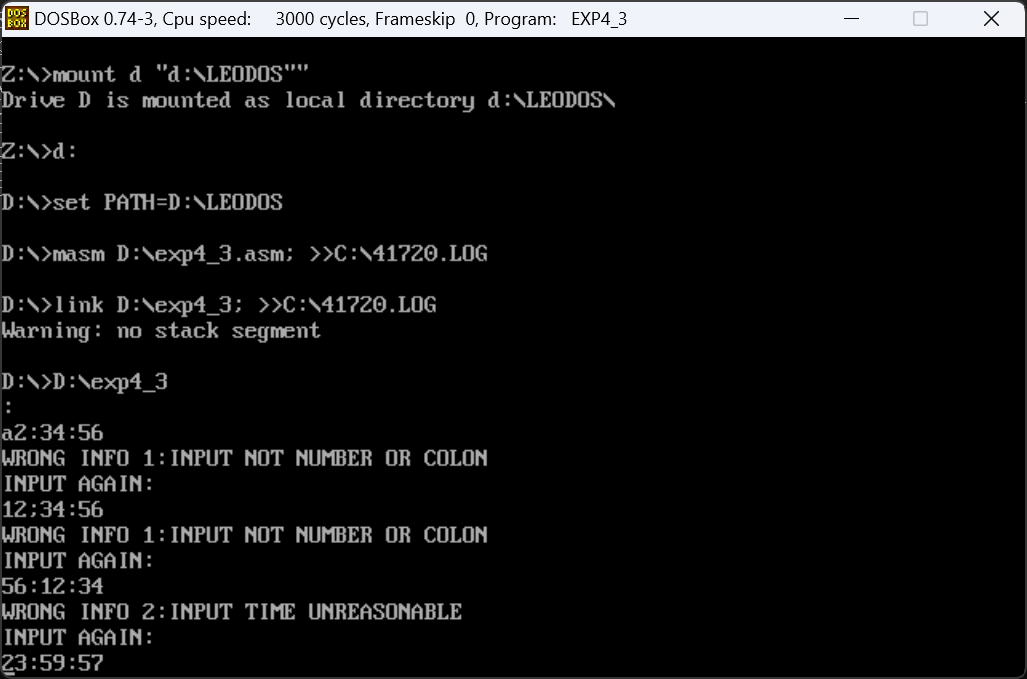
\includegraphics[scale=0.48]{pic/exp4-2-correctinput.png}
    \caption{附加实验任务结果截图2}
    \label{附加实验任务结果截图2}
    \end{minipage}
\end{figure}
\begin{figure}[H]
    \centering
    \begin{minipage}{0.45\textwidth}
    \centering
    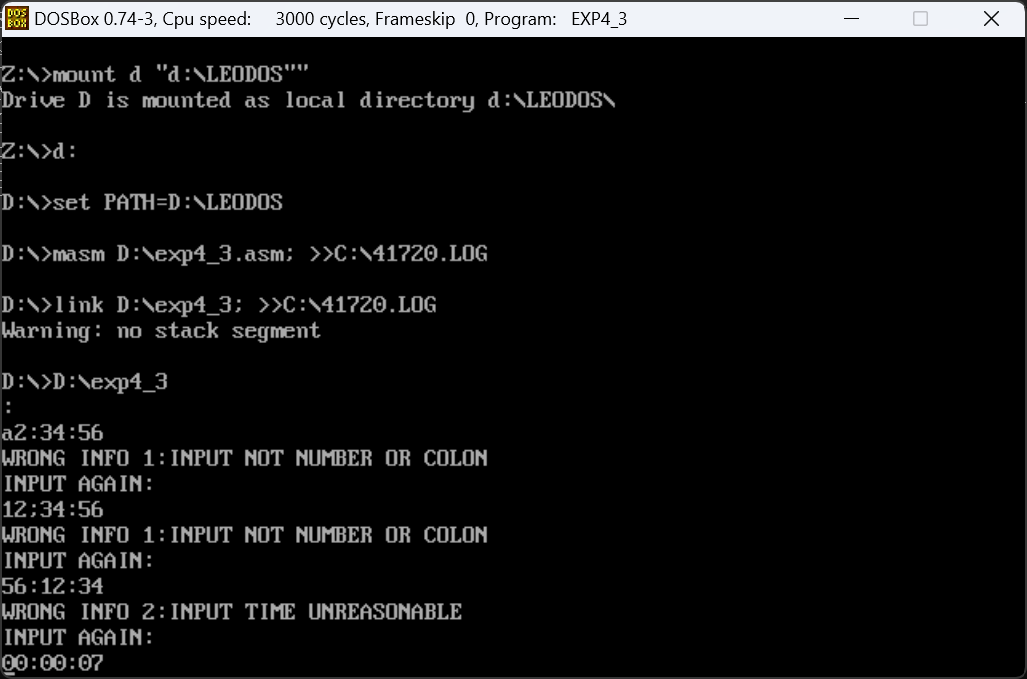
\includegraphics[scale=0.48]{pic/exp4-2-counting.png}
    \caption{附加实验任务结果截图3}
    \label{附加实验任务结果截图3}
    \end{minipage}
    \hspace{0.05\textwidth}
    \begin{minipage}{0.45\textwidth}
    \centering
    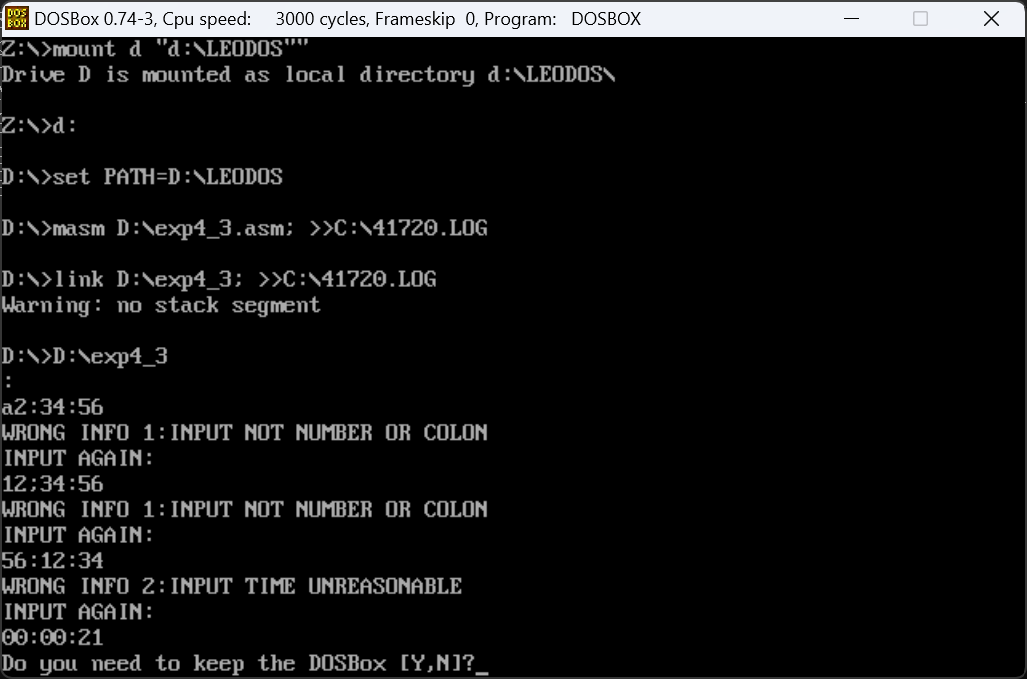
\includegraphics[scale=0.48]{pic/exp4-2-end.png}
    \caption{附加实验任务结果截图4}
    \label{附加实验任务结果截图4}
    \end{minipage}
\end{figure}
\section{实验总结}
在完成基础任务时,遇到以下问题:
\begin{enumerate}
    \item 没有理解0DH和0AH的作用,光标位置不在预想的位置。0DH使光标移到行首,0AH换行。要输出更新后的时间之前,应该先换行,否则会覆盖之前的输出。
    \item 编写子程序的时候,最初没有保护现场,导致寄存器的值被改变,程序崩溃。解决方法是:编写子程序时先将可能改变的寄存器入栈,子程序结束后再出栈恢复现场。
    \item 编写延时程序时,最开始有一步设置了系统时间,后来发现这一步是不必要的,且系统时间也不应该修改,遂删去。
\end{enumerate}
在完成附加任务时,遇到以下问题:
\begin{enumerate}
    \item 为了增加代码复用性,将ASCII码到BCD码的转换写成子程序(ATOB),但是在结尾处忘了写RET,结果每次调用ATOB后程序会顺次执行下面的DELAY子程序,导致每次延时都会多1秒。加上RET后恢复正常。
    \item 编写检查子程序(CHECK)时,最初用到AX来做指针指向每一个待检查的字符,但发现编译结果总与预想不同。上网查阅发现AX,CX,DX均不能存放地址。于是改用BX,使问题得到解决。
    \item 编写检查程序时,发现即使输入正确也会打印第一类错误信息。经检查,是因为在经过所有检查流程(即输入正确)后,没有加跳转到子程序出口的指令。而此处后面正好跟的是输出第一类错误信息的程序,所以会出现错误。解决办法:加上JMP OVER,使得经过所有检查流程直接跳转到子程序出口。
\end{enumerate}
\section{思考题}
时钟程序中存在时间误差吗? 若有误差,其来源在何处? 如何进行误差校正?

答:存在误差。来源于程序本身运行的耗时和延时程序的误差。其中后者是主要误差来源。本程序中,延时子程序的逻辑是:读取系统时间,将秒值加1,再次读取系统时间,并将新读出的秒值与加1后的结果比较,如果不同,则再次读取如此循环,如果相同,说明距离第一次读取(即进入延时程序的瞬间)已经过去一秒,这时退出延时子程序。这种延时可能会在首次调用该子程序时有较大误差。

这种延时的缺陷在于,仅检查了秒值。忽略计算机执行耗时,假若第一次读取系统时间为00:00:00 50ms,则在00:00:01 00ms瞬间就会退出延时,延时不足1秒。若考虑计算机执行的耗时,则会出现新的误差。在延时程序以外,不能保证每次其他部分的程序都执行1秒的整数倍。否则由于同样的原因,除了首次调用,后续每一次调用都会产生误差。改进办法是同时检查秒值与毫秒值,仅当秒值与初始秒值加一后的结果相同且毫秒值也相同的时候才退出。
\end{document}